\chapter{Controllo $H_\infty$: baseline e revisione mirata}
\label{cap:hinf}
\section{Obiettivo energetico e mappe della retroazione}
Il controllo $H_\infty$ cerca un regolatore che limiti il peggiore guadagno
delle mappe di interesse. Per una matrice di trasferimento stabile $F$,
\[
\|F\|_\infty=\sup_{\omega\in\mathbb R}\bar\sigma(F(j\omega))
=\sup_{0<\|w\|_2<\infty}\frac{\|z\|_2}{\|w\|_2},\qquad z=Fw.
\]
Si considera quindi la peggiore frequenza e la peggiore direzione MIMO
dell'ingresso, non la media dei due giunti. L'interpretazione energetica
riguarda ingressi a energia finita. Un gradino permanente non è in $L_2$:
settling, overshoot e picco istantaneo di coppia devono essere verificati
separatamente, non dedotti automaticamente dalla norma.

Per la pianta M3, $G:u\mapsto q$ ha dimensione $2\times2$, 14 stati,
ingressi in N m e uscite in rad. Il regolatore riceve $e=r-q$ e produce
$u=Ke$. Definiamo le mappe all'uscita
\[
S=(I+GK)^{-1},\qquad
T=GK(I+GK)^{-1}=I-S,\qquad
KS=K(I+GK)^{-1}.
\]
$S$ collega riferimento ed errore, $T$ riferimento e posizione,
$KS$ riferimento e comando. Un rumore additivo di misura si trasmette
alla posizione mediante $-T$ e al comando mediante $-KS$.
Per la coppia disturbante lato link, invece, la mappa fisica è
$SG_d$: non basta chiamare $S$ la risposta a qualsiasi disturbo.

LQG e $H_\infty$ rispondono a problemi diversi. M6 impiega una stima
dello stato basata su $q,\theta$ e ipotesi statistiche sui rumori;
la sintesi qui studiata utilizza soltanto i due errori di posizione $r-q$
e minimizza un criterio frequenziale worst-case. Non riutilizza $K$ o $L$
di M6 e non dispone automaticamente delle stesse prestazioni.

\section{Pesi originali M5: significato e audit delle unità}
La configurazione originaria usa
\[
W_1(s)=\frac{s/2+12}{s+0.6}I_2,\qquad
W_2(s)=\frac1{12}\frac{s/30+1}{s/180+1}I_2,\qquad W_3=\varnothing.
\]
$W_1(0)=20$ traduce l'obiettivo di sensibilità statica $A_s=0.05$;
$W_1(\infty)=0.5$ corrisponde al parametro $M_s=2$.
Il polo è $0.6$, lo zero $24$ e la frequenza $|W_1|=1$ è
$13.839$ rad/s: $\omega_B=12$ è un parametro di transizione,
non una misura della banda effettivamente ottenuta.
$W_2$ ha guadagno DC $1/12$, guadagno asintotico $0.5$,
zero $30$ e polo $180$ rad/s. Non attraversa il livello uno.

La simmetria dei due pesi è coerente con le medesime unità e scale
dei due giunti, ma non rende isotropa la pianta: a 12 rad/s i valori
singolari di $G$ sono circa $0.1713$ e $0.0101$ rad/(N m).
La direzione meno controllabile in frequenza richiede un comando
molto maggiore a parità di uscita.

Il prodotto $W_2KS$ della baseline agisce sul guadagno da un riferimento
espresso numericamente in rad al comando. Non impone direttamente
$|u(t)|\leq12$ N m per il gradino di 5 gradi.
La scala di riferimento implicita è 1 rad, non $q_s=5\pi/180$ rad.
Questo non rende falso il vecchio problema matematico: ne rende il costo
di comando più restrittivo rispetto a un problema esplicitamente
normalizzato sul caso M5 da 5 gradi. Correggere l'interpretazione delle
unità non autorizza a presentare una norma $L_2$ come limite di picco.

Anche la traduzione temporale è una scelta di loop shaping, non
un'equivalenza: imporre un inviluppo su $S$ con $A_s,M_s,\omega_B$
non garantisce da solo $T_s\leq0.8$ s e overshoot $\leq10\%$.
Il modello comprende inoltre poli instabili a circa $4.0408$ e
$7.2094$ s$^{-1}$, dinamica attuativa con $\omega_n=40$ rad/s,
ritardo nominale 15 ms e due zeri di Padé nel semipiano destro
a $133.333$ s$^{-1}$. Questi elementi vincolano la stabilizzazione
e il compromesso di banda; non sono eliminati dalla normalizzazione.

\subsection{Una incompatibilità verificabile prima del retuning}
Con pesi scalari replicati sui due giunti, poniamo
$a=|W_{1,\mathrm{siso}}(j\omega)|$,
$b=|W_{2,\mathrm{siso}}(j\omega)|$ e
$g=\underline\sigma(G(j\omega))$. Poiché $S+GKS=I$, persino
rilassando il problema e scegliendo liberamente il comando complesso
a ogni frequenza, il costo nella direzione meno efficace non può
scendere sotto
\[
\gamma\ \geq\
\sup_\omega \frac{a(\omega)b(\omega)}
{\sqrt{b(\omega)^2+a(\omega)^2g(\omega)^2}}.
\]
Il limite deriva dalla minimizzazione quadratica puntuale di
$a^2|1-gv|^2+b^2|v|^2$ rispetto al comando $v$.
Non impone causalità o stabilità del controllore: è una condizione
necessaria, non una formula per il controllore ottimo.

Con i pesi originali il valore calcolato sulla griglia è almeno
$1.645$ a circa $5.754$ rad/s. Esiste quindi già un conflitto fra
i due inviluppi che esclude $\gamma<1$, indipendentemente dall'algoritmo
di sintesi. Non spiega da solo l'intero valore $10.207$:
i vincoli dinamici e di stabilità interna rendono il problema completo
più restrittivo del rilassamento puntuale.

\section{M9 e M10: conservazione della baseline a due pesi}
M9 risolve
\[
\min_K\left\|\begin{bmatrix}W_1S\\W_2KS\end{bmatrix}\right\|_\infty
\]
con \texttt{mixsyn}. Il controllore è di ordine 18 e nominalmente
stabile, ma $\gamma=\MixsynGamma>1$.
I due contributi sono circa $10.128$ e $10.185$.
Il massimo di $W_1S$ è in DC; quello di $W_2KS$ è intorno a
$33.44$ rad/s, vicino alla dinamica attuativa. Entrambi gli inviluppi
sono violati, non uno soltanto.

M10 costruisce invece esplicitamente, con \texttt{connect} e
\texttt{sumblk}, i segnali
$e=r-q$, $z_1=W_1e$, $z_2=W_2u$:
\[
\begin{bmatrix}z_1\\z_2\\e\end{bmatrix}
=
\underbrace{\begin{bmatrix}
W_1&-W_1G\\0&W_2\\I&-G
\end{bmatrix}}_{P}
\begin{bmatrix}r\\u\end{bmatrix}.
\]
Qui $w=r\in\mathbb R^2$ è l'ingresso esogeno,
$z=[z_1^T,z_2^T]^T\in\mathbb R^4$ l'uscita prestazionale,
$y=e\in\mathbb R^2$ la misura fornita al controllore e
$u\in\mathbb R^2$ il comando. Nell'ordine richiesto da
\texttt{hinfsyn}, le misure sono le ultime uscite e i comandi gli
ultimi ingressi. La pianta è quindi $6\times4$.

Partizionando $P$ secondo $[z;y]$ e $[w;u]$, la lower LFT è
\[
F_\ell(P,K)=P_{11}+P_{12}K(I-P_{22}K)^{-1}P_{21}.
\]
Il segno negativo della retroazione è già contenuto in $P_{22}=-G$:
non va aggiunto un secondo cambio di segno.
La chiamata \texttt{hinfsyn(P,2,2)} e \texttt{mixsyn(G,W1,W2,[])}
rappresentano lo stesso problema quando pesi e segnali coincidono.
M10 ne verifica l'equivalenza, ottenendo ordine \KhinfOrder\
e $\gamma=\HinfsynGamma$.

\begin{figure}[htbp]\centering
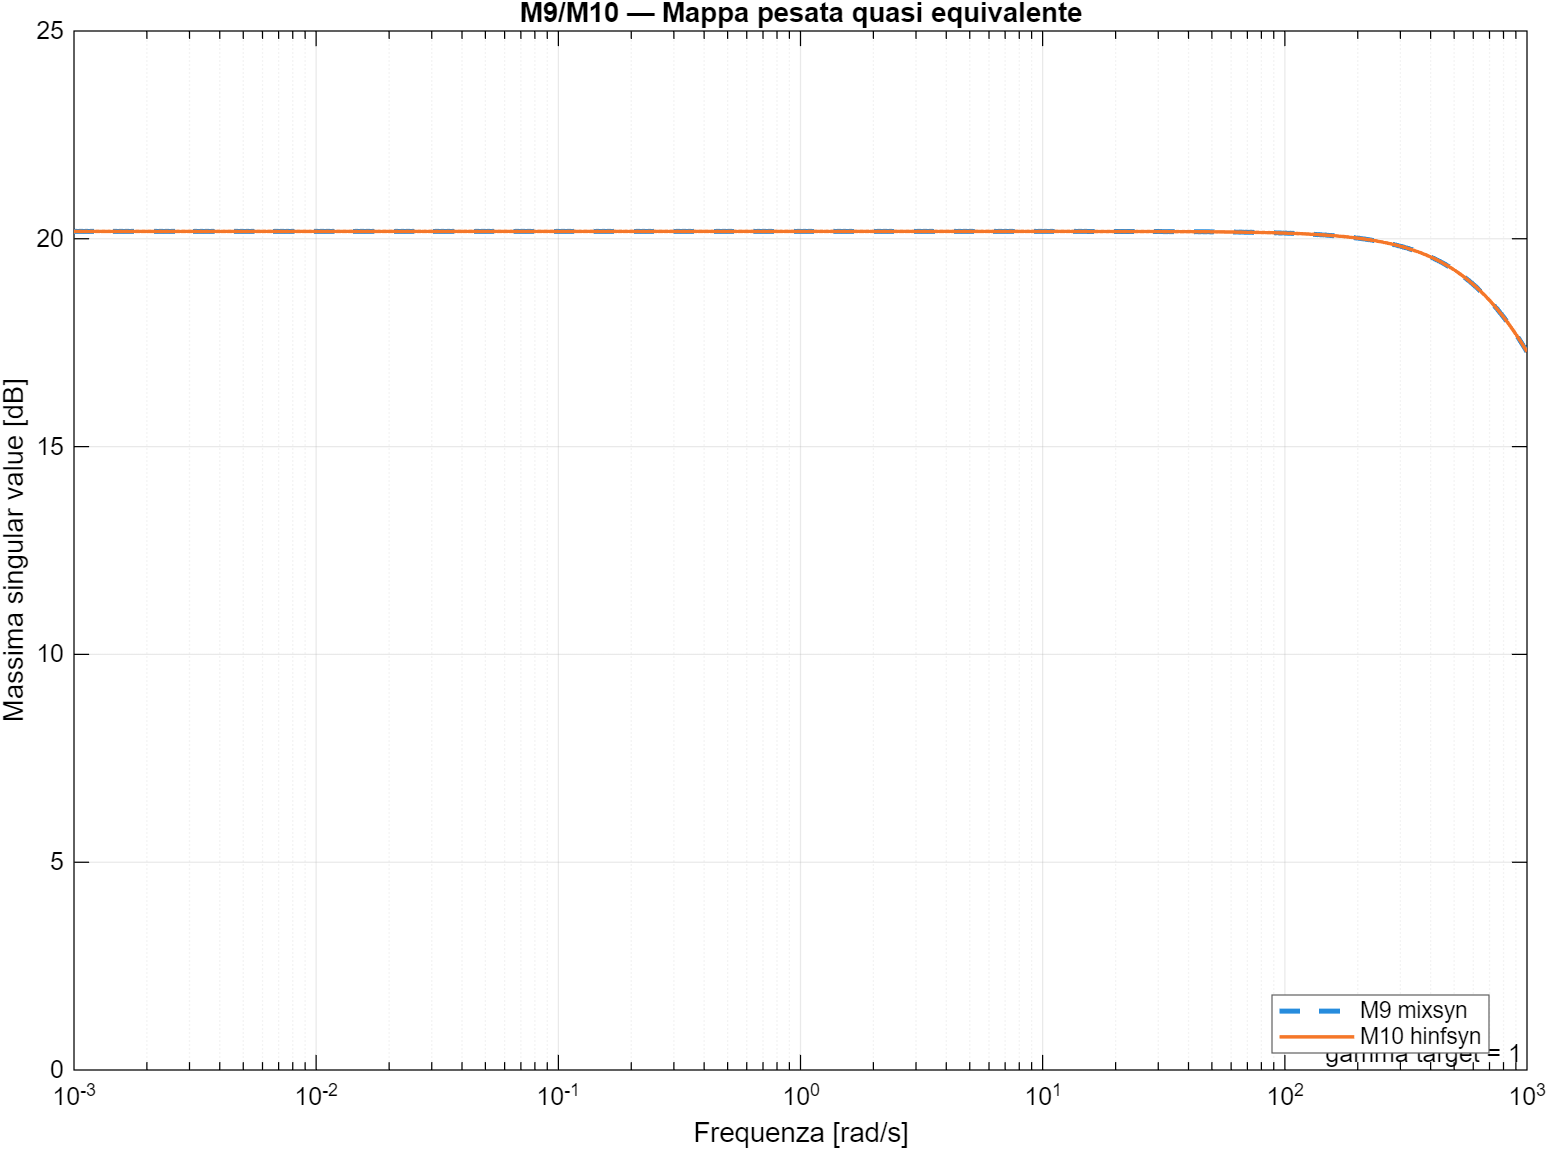
\includegraphics[width=0.88\textwidth]{figures/m10_weighted_comparison_m9.png}
\caption{Baseline originale M9/M10: la sovrapposizione delle mappe verifica l'equivalenza delle interconnessioni, non il soddisfacimento del target uno.}
\label{fig:m10-weighted}
\end{figure}
La Figura~\ref{fig:m10-weighted} conserva il risultato iniziale.
Non vengono sovrascritti gli artifact M9 o M10 e non si introduce
un prefiltro per alterarne retroattivamente le risposte.

\section{Revisione motivata: normalizzazione e terzo canale}
\subsection{Separare cambio di unità e cambio del requisito pesato}
Nel nuovo studio si definiscono
\[
r_N=r/q_s,\quad q_N=q/q_s,\quad u_N=u/u_s,\qquad
G_N=\frac{u_s}{q_s}G,\quad q_s=5\pi/180,\quad u_s=12.
\]
Il controllore fisico è $K=(u_s/q_s)K_N$.
Un puro cambio di coordinate, con tutti i pesi trasformati in modo
equivalente, mantiene la vecchia norma $10.207$; questo viene controllato.
La modifica progettuale è invece adottare
\[
W_{2,N}(s)=\beta_U\frac{s/30+1}{s/180+1}I_2,\qquad
W_{2,\mathrm{fisico}}=\frac{q_s}{u_s}W_{2,N}.
\]
Per $\beta_U=1$ si confrontano il riferimento normalizzato da 5 gradi
e il comando normalizzato su 12 N m. È un rilassamento dichiarato del
peso fisico rispetto alla baseline, non una semplice riscrittura
equivalente. Per $\beta_U=2$ la penalità di comando raddoppia.
La prova diagnostica ID 1 modifica soltanto questa scala e mantiene
$W_1$ e l'assenza di $W_3$: $\gamma$ scende a circa $3.448$,
ma resta maggiore di uno.

\subsection{Perché introdurre \texorpdfstring{$W_3T$}{W3T}}
Un peso su $T$ permette di richiedere attenuazione del rumore di misura
alle alte frequenze e roll-off dell'uscita prima delle dinamiche poco
affidabili. Nel progetto esistono attuatori finiti, un'approssimazione
Padé e rumore encoder, ma non un inviluppo quantitativo del docente
che determini univocamente $W_3$.

La scelta del nuovo studio è pertanto esplicitamente progettuale:
\[
W_3(s)=\frac{s/\omega_T+0.1}{s/(5\omega_T)+1}I_2,\qquad
\omega_T\in\{40,80\}\ {\rm rad/s}.
\]
Il guadagno DC è $0.1$, quello ad alta frequenza è 5.
Lo zero è $0.1\omega_T$, il polo è $5\omega_T$ e il crossover
è $\omega_T\sqrt{0.99/0.96}$, circa $1.0155\omega_T$.
I due valori collocano la transizione presso $\omega_n$ oppure
$2\omega_n$: una richiesta più precoce e una meno restrittiva.
Non sono un'identificazione dello spettro di rumore.

Il peso d'incertezza $W_I$ di M4 descrive invece perturbazioni
moltiplicative all'ingresso degli attuatori. Nel caso MIMO
la complementarità d'ingresso è $T_i=KG(I+KG)^{-1}$ e non coincide
in generale con $T=GK(I+GK)^{-1}$. Perciò usare direttamente
$W_I$ come peso di $T$ non fornirebbe automaticamente il certificato
M4. Il nuovo $W_3$ è un peso di progetto nominale; la $\mu$-analysis
rimane una verifica separata.

\subsection{Campagna deterministica e criteri dichiarati}
Si mantengono $A_s=0.05$, $M_s=2$, $\omega_U=30$,
$\alpha=6$ e tutti i target temporali M5.
La campagna incrocia
\[
\omega_B\in\{8,12,16\},\quad
\beta_U\in\{1,2\},\quad \omega_T\in\{40,80\}.
\]
Le tre bande sono $\omega_n/5$, $0.3\omega_n$, $0.4\omega_n$:
inquadrano una richiesta meno aggressiva, quella originale e una più
aggressiva, senza fingere che la prima garantisca il settling M5.
Sono 12 candidati a tre pesi, più il diagnostico ID 1 senza $W_3$.
Si eseguono inoltre una verifica \texttt{hinfsyn} equivalente sul candidato
illustrativo e una sintesi diagnostica con il solo peso di comando:
15 sintesi in totale, non una ricerca casuale.

Il diagnostico sul solo comando normalizzato restituisce circa
$0.4081$, ma non impone tracking e non è un'alternativa utilizzabile.
Mostra che non è corretto attribuire il mancato $\gamma<1$
alla sola penalizzazione del comando: conta il compromesso con $W_1$,
la stabilizzazione e, quando presente, $W_3$.

Ogni candidato viene valutato su stabilità della matrice plant--controller
completa, norma dello stack, tre norme componenti, due gradini da 5 gradi,
settling, overshoot, errore statico, cross-coupling, picco e RMS di comando.
La selezione illustrativa considera solo candidati a tre pesi stabili
e ordina lessicograficamente: eventuale $\gamma<1$, numero di target M5
violati, massimo rapporto fra metrica temporale e target, picco relativo
di comando, cross-coupling, infine $\gamma$. Non vi è uno score nascosto.
Poiché tutti violano i tre target, il candidato ID 10 viene scelto
per il confronto temporale; non è quello a $\gamma$ minimo e non è
promosso a controllore finale.

\begin{table}[htbp]\centering\small
\begin{tabular}{p{2.1cm}p{3.1cm}p{3.1cm}p{5.1cm}}\toprule
Parametro & Originale & Illustrativo ID 10 & Motivazione \\\midrule
$W_1$: $A_s,M_s$ & $0.05,2$ & invariati & Nessun rilassamento dell'obiettivo statico o del parametro di picco \\
$W_1$: $\omega_B$ & 12 & 16 rad/s & Estremo più aggressivo della terna, scelto dal criterio temporale dichiarato \\
$W_2$: scala & $1/12$ & $(5\pi/180)/12$ & Confronto fra riferimento da 5 gradi e comando da 12 N m, dichiaratamente meno restrittivo \\
$W_2$: zero/polo & $30/180$ & invariati & Stessa penalizzazione relativa dei comandi rapidi \\
$W_3$ & assente & DC 0.1, HF 5, $\omega_T=40$ & Roll-off nominale presso la dinamica attuativa; scelta del progetto \\\bottomrule
\end{tabular}
\caption[Revisione motivata dei pesi]{Modifiche del problema pesato, non dei target temporali M5 o dell'insieme incerto M4.}
\label{tab:hinf-pesi-nuovi}
\end{table}

\subsection{Pianta generalizzata a tre pesi e verifiche indipendenti}
Con i segnali normalizzati, $z_3=W_3q_N$ si aggiunge agli altri
due canali:
\[
P_N=
\begin{bmatrix}
W_1&-W_1G_N\\
0&W_{2,N}\\
0&W_3G_N\\
I&-G_N
\end{bmatrix},\qquad
F_\ell(P_N,K_N)=
\begin{bmatrix}W_1S\\W_{2,\mathrm{fisico}}KS\\W_3T\end{bmatrix}.
\]
La pianta è $8\times4$: sei uscite prestazionali, due misure,
due ingressi esogeni e due comandi. \texttt{connect} usa una sola
istanza di $G_N$. La formula a blocchi e \texttt{augw} sono confronti
indipendenti in frequenza; la lower LFT viene confrontata con lo stack
ricostruito dalla chiusura fisica. \texttt{mixsyn} e
\texttt{hinfsyn(PN,2,2)} restituiscono objective coerenti.
Il numero $\gamma<1$ avrebbe significato solo rispetto a questi pesi
normalizzati, non rispetto a qualsiasi requisito fisico o alla robustezza M4.

\section{Risultati del nuovo studio e figure didattiche}
% Generated by plot_hinf_revision.m.
\begin{table}[htbp]\centering\small
\begin{tabular}{rrrrrrrr}\toprule
ID & $\omega_B$ & $\beta_U$ & $\omega_T$ & $\gamma$ & OS [\%] & picco $u$ & stabili/5 \\\midrule
0 & 12 & 11.459 & 0 & 10.207 & 261.62 & 5.1599 & 5 \\
1 & 12 & 1 & 0 & 3.4477 & 155.9 & 14.19 & 2 \\
2 & 8 & 1 & 40 & 2.8302 & 149.13 & 11.859 & 3 \\
3 & 8 & 1 & 80 & 2.8056 & 152.82 & 11.956 & 3 \\
4 & 8 & 2 & 40 & 3.6641 & 180.56 & 8.7844 & 4 \\
5 & 8 & 2 & 80 & 3.6476 & 186.15 & 8.829 & 4 \\
6 & 12 & 1 & 40 & 3.4886 & 145.41 & 13.952 & 3 \\
7 & 12 & 1 & 80 & 3.4624 & 151.62 & 14.069 & 2 \\
8 & 12 & 2 & 40 & 4.4659 & 175.43 & 10.222 & 3 \\
9 & 12 & 2 & 80 & 4.4561 & 180.17 & 10.297 & 3 \\
10 & 16 & 1 & 40 & 4.073 & 144.44 & 15.686 & 2 \\
11 & 16 & 1 & 80 & 4.0464 & 153.38 & 15.818 & 2 \\
12 & 16 & 2 & 40 & 5.1858 & 169.39 & 11.438 & 3 \\
13 & 16 & 2 & 80 & 5.1687 & 173.44 & 11.51 & 3 \\
\bottomrule\end{tabular}
\caption{Campagna deterministica. ID 0 è la baseline ricaricata; ID 1 isola la nuova scala di comando senza $W_3$. Le frequenze sono in rad/s, il comando in N m. Tutti sono nominalmente stabili; nessuno supera tutti i target M5. I cinque campioni M4 non certificano robustezza.}
\label{tab:hinf-campagna}\end{table}
\begin{table}[htbp]\centering\small
\begin{tabular}{lrr}\toprule
Metrica & M10 originale & candidato illustrativo \\\midrule
$\gamma$ & 10.207 & 4.073 \\
$\|W_1S\|_\infty$ & 10.128 & 4.0702 \\
$\|W_2KS\|_\infty$ & 10.185 & 4.0339 \\
$\|W_3T\|_\infty$ & 0 & 2.5921 \\
$T_s$ [s] & 1.566 & 1.162 \\
Overshoot [\%] & 261.62 & 144.44 \\
Errore statico relativo & 0.49068 & 0.20143 \\
Cross-coupling & 0.2596 & 0.19912 \\
Picco comando [N m] & 5.1599 & 15.686 \\
RMS comando [N m] & 1.0517 & 1.1913 \\
Ordine & 18 & 20 \\
\bottomrule\end{tabular}
\caption{Metriche peggiori fra due gradini nominali separati da 5 gradi, 12 s, senza disturbi o rumore. I valori $\gamma$ riguardano problemi pesati diversi: non sono direttamente una graduatoria di robustezza.}
\label{tab:hinf-nuovo-confronto}\end{table}

Il miglior $\gamma$ della campagna è circa $2.806$ (ID 3);
nessun candidato raggiunge uno. Il candidato illustrativo ID 10 ha
$\gamma\simeq4.073$, $T_s=1.162$ s, overshoot $144.44\%$ e
picco di comando $15.686$ N m. Il miglioramento rispetto alla baseline
non rende questi valori accettabili. Le norme di problemi pesati
diversi non costituiscono da sole una misura comparabile di qualità.

La Figura~\ref{fig:hinf-pesi-rivisti} mostra le modifiche ai pesi.
La Figura~\ref{fig:hinf-inviluppi} risponde invece alla domanda
se le due direzioni singolari di $S$ e $T$ rispettino gli inviluppi
scelti. Il confronto scalare è corretto perché ogni peso è un filtro
scalare replicato sui due canali, non una matrice arbitraria.
\begin{figure}[htbp]\centering
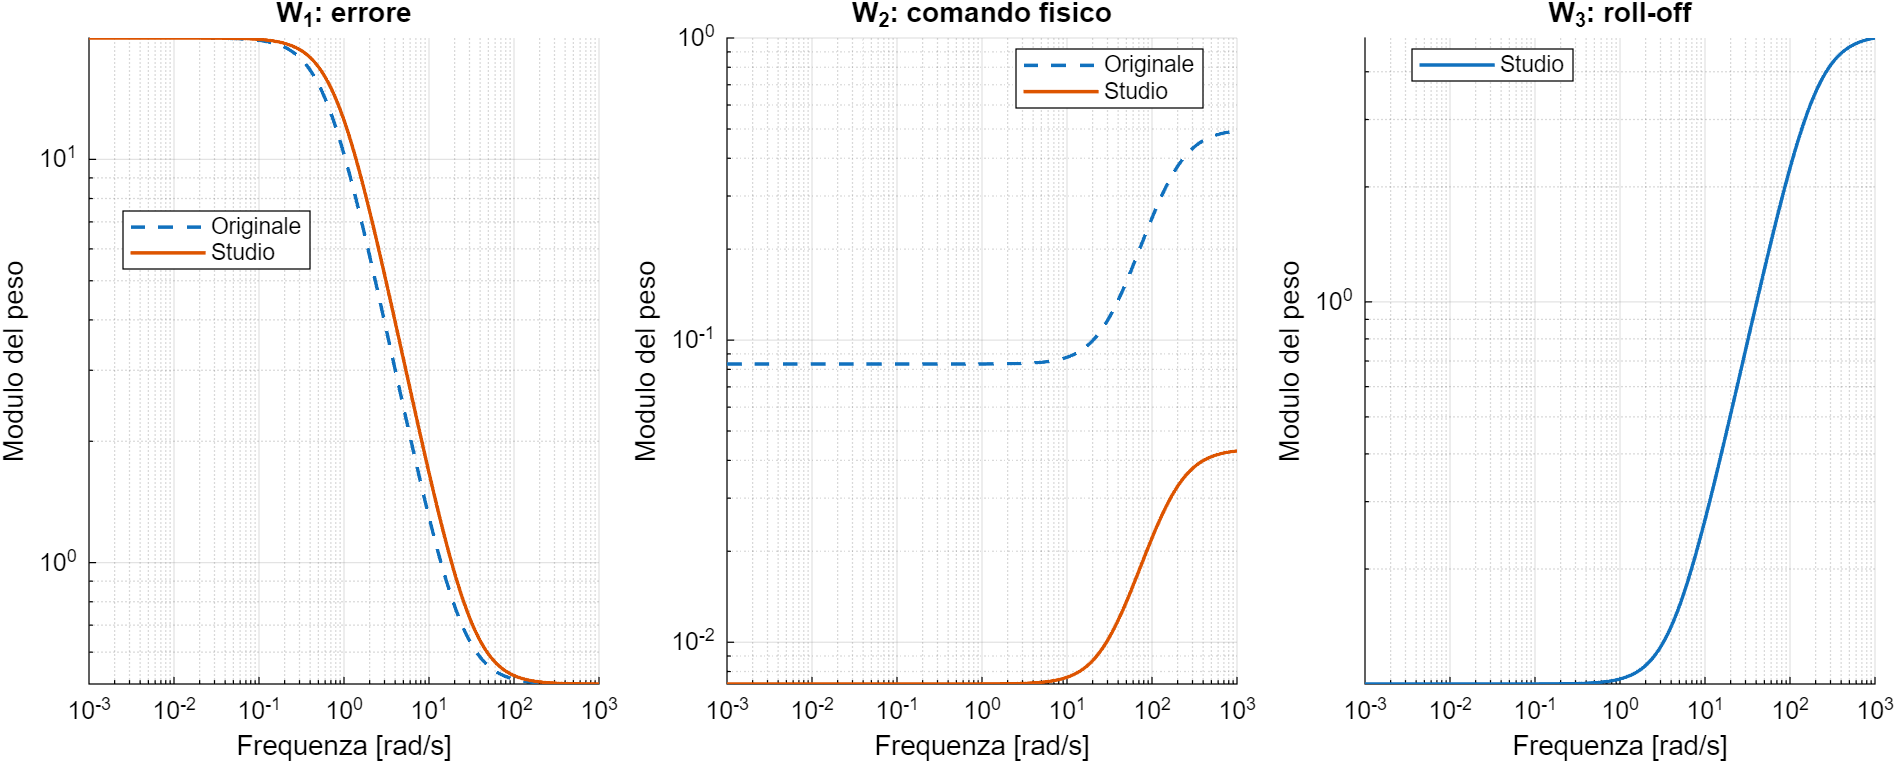
\includegraphics[width=0.98\textwidth]{figures/hinf_revision_weights.png}
\caption{Pesi fisici originali e del candidato ID 10. Il vecchio $W_3$ è assente, non un filtro non nullo nascosto sotto il grafico.}
\label{fig:hinf-pesi-rivisti}
\end{figure}
\begin{figure}[htbp]\centering
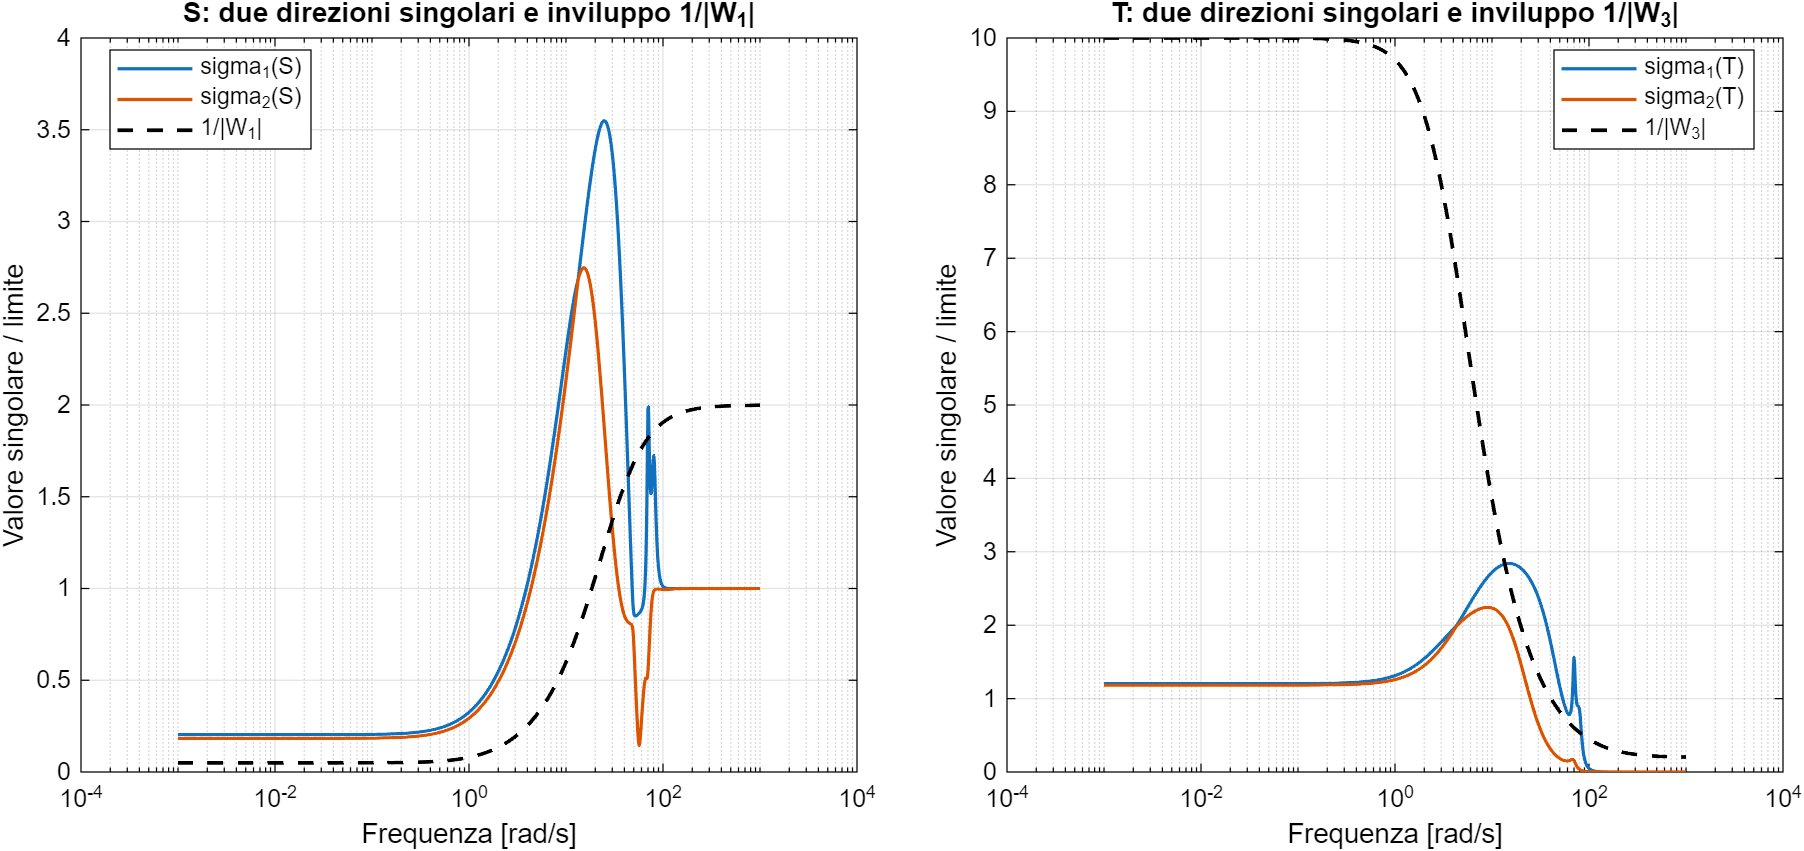
\includegraphics[width=0.96\textwidth]{figures/hinf_revision_sensitivity_envelopes.png}
\caption{Valori singolari di $S$ e $T$ confrontati rispettivamente con $1/|W_1|$ e $1/|W_3|$. Gli inviluppi sono obiettivi del nuovo problema, non certificati di robustezza.}
\label{fig:hinf-inviluppi}
\end{figure}

La Figura~\ref{fig:hinf-canali-rivisti} espone direttamente i tre
contributi e il livello uno. La norma dello stack non è semplicemente
il massimo delle tre norme: i canali si sommano quadraticamente
nella matrice prestazionale prima della massimizzazione.
\begin{figure}[htbp]\centering
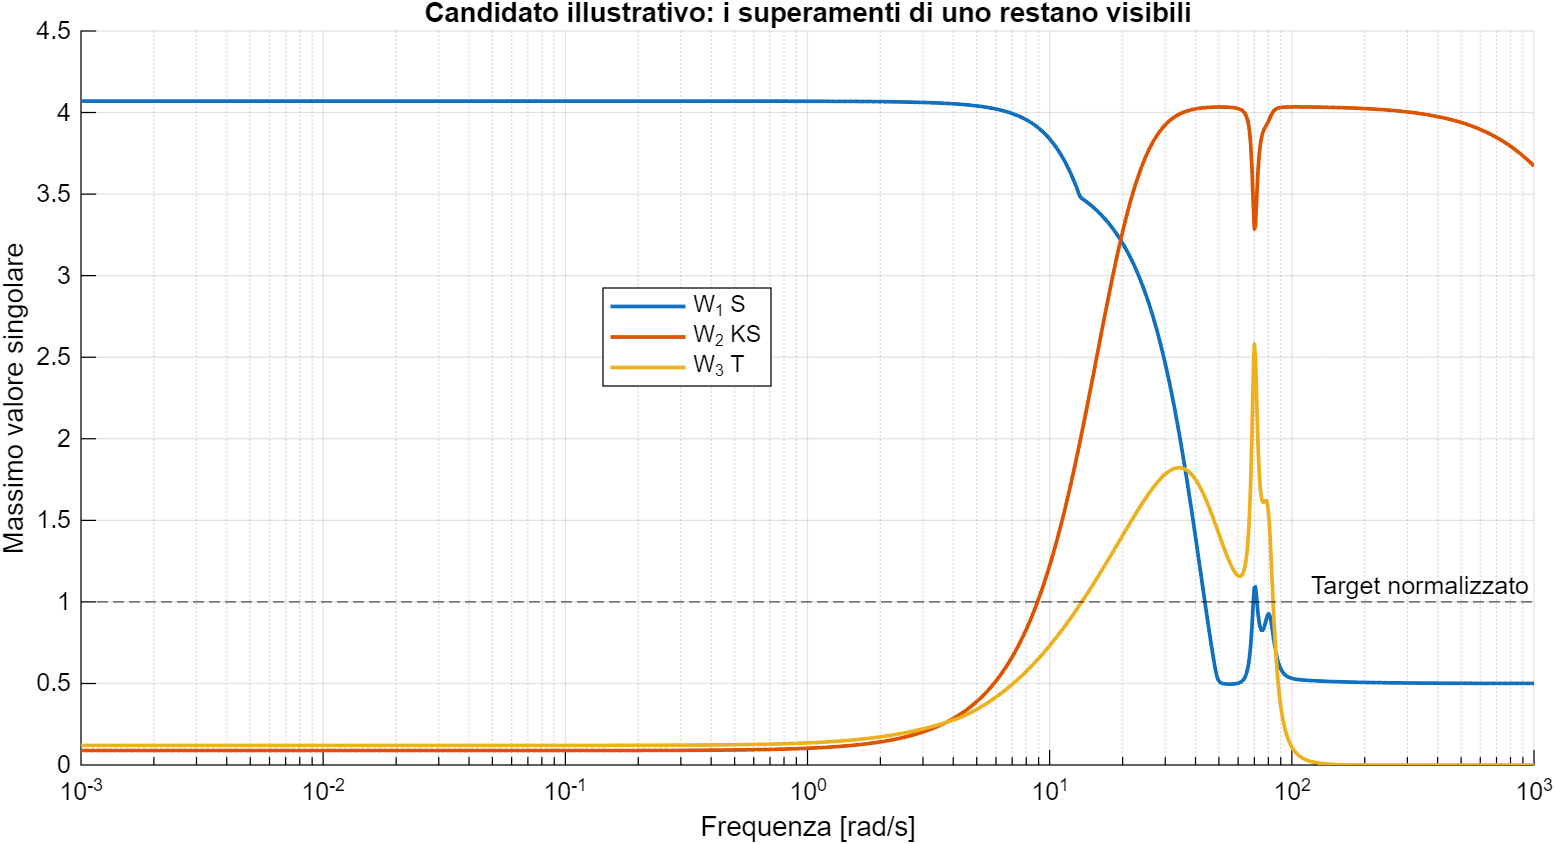
\includegraphics[width=0.86\textwidth]{figures/hinf_revision_weighted_channels.png}
\caption{Massimi valori singolari di $W_1S$, $W_2KS$, $W_3T$ per ID 10. Tutti i superamenti del target sono conservati.}
\label{fig:hinf-canali-rivisti}
\end{figure}
La Figura~\ref{fig:hinf-tempo-rivisto} mostra due esperimenti separati
con stesso orizzonte di 12 s, stato nullo, nessun disturbo o rumore.
Le colonne distinguono il giunto di riferimento, le righe posizioni
e comandi. L'overshoot molto elevato e l'offset finale spiegano
perché il risultato non venga selezionato come controllore del progetto.
\begin{figure}[htbp]\centering
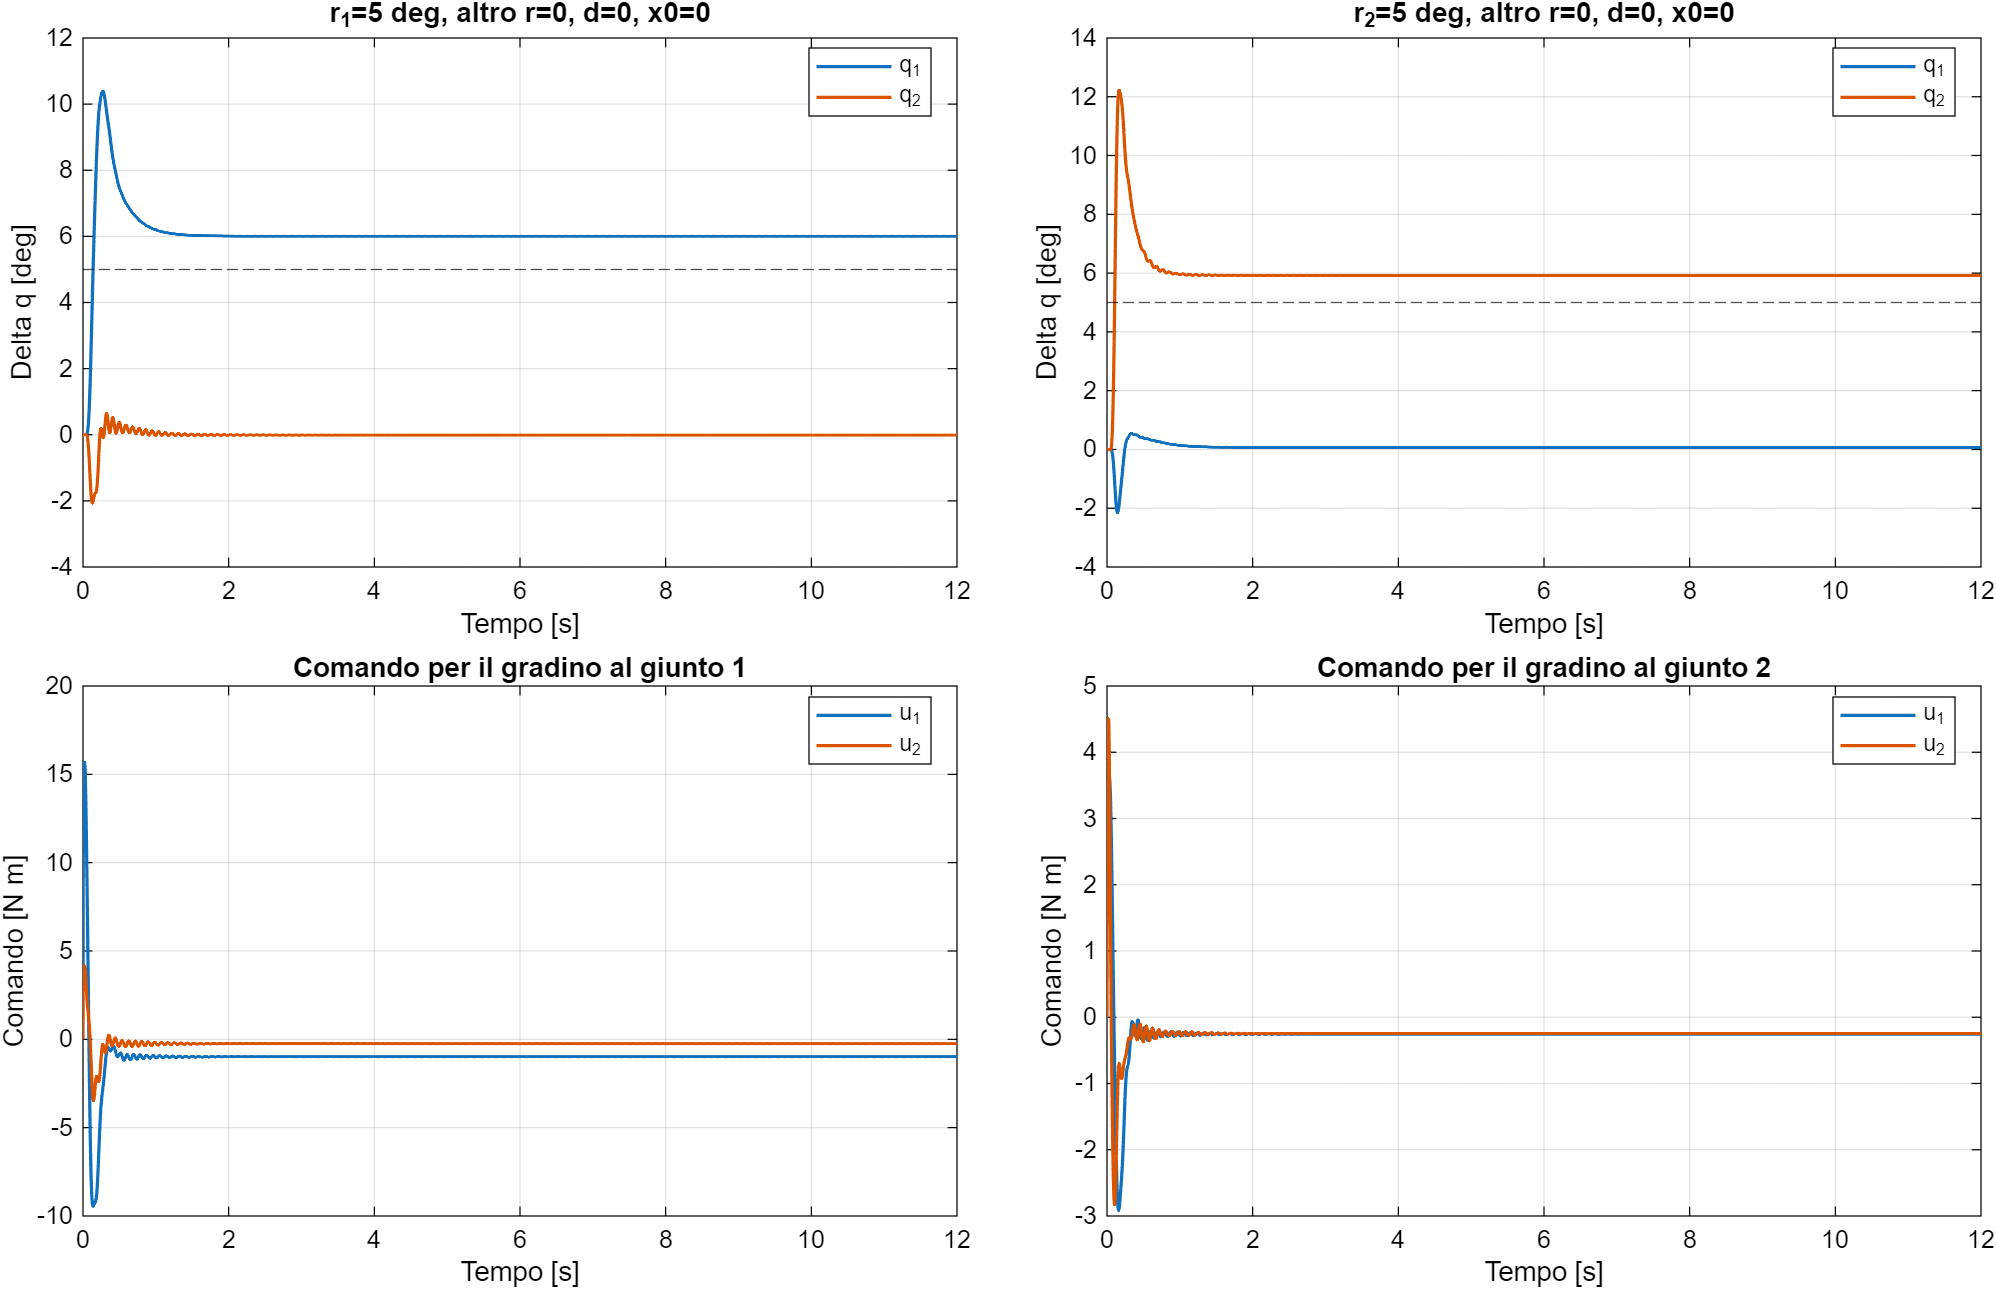
\includegraphics[width=0.95\textwidth]{figures/hinf_revision_tracking_control.png}
\caption{Tracking e comando di ID 10 per gradini da 5 gradi. La linea tratteggiata indica il riferimento del giunto eccitato; l'altro riferimento è nullo. Nessun prefiltro o saturazione è aggiunto.}
\label{fig:hinf-tempo-rivisto}
\end{figure}

Cinque campioni M4 comuni, seed 20260910, completano il controllo
esplorativo: ID 10 è stabile soltanto in 2/5 casi, mentre la baseline
M10 lo è in 5/5. Non sono i 40 campioni ufficiali M16 e le frazioni
non sono probabilità o certificati. Non emerge pertanto una ragione
per sostituire la baseline robusta con il nuovo candidato.

\section{M11: full-order, strutture implementabili e analisi successive}
Il controllore full-order viene ottenuto senza imporre a priori
una struttura a basso ordine. Il nuovo problema a tre pesi produce
ordine 20, contro 18 della baseline: si aggiungono due stati di peso.
Un ordine maggiore aumenta la libertà dinamica, ma non garantisce
automaticamente un miglior risultato utile o una maggiore robustezza.

M11 rimane lo studio strutturato del problema originale, non viene
rinominato come risultato dei nuovi pesi. Comprende guadagno statico
MIMO, due PI decentralizzati, due PID filtrati e tre strutture MIMO
di ordine 2, 4, 6, con cinque partenze per famiglia.
A0/A1 non producono objective finiti, A2 non produce chiusure stabili;
A3/A4/A5 danno cinque soluzioni stabili ciascuna. I migliori objective
sono circa $16.6419$, $11.6555$ e \AFiveGamma.
La maggiore flessibilità riduce il divario dal full-order, a costo
di più stati e parametri. Le ottimizzazioni strutturate non sono
necessariamente globali: le partenze multiple documentano questo limite.

\begin{figure}[htbp]\centering
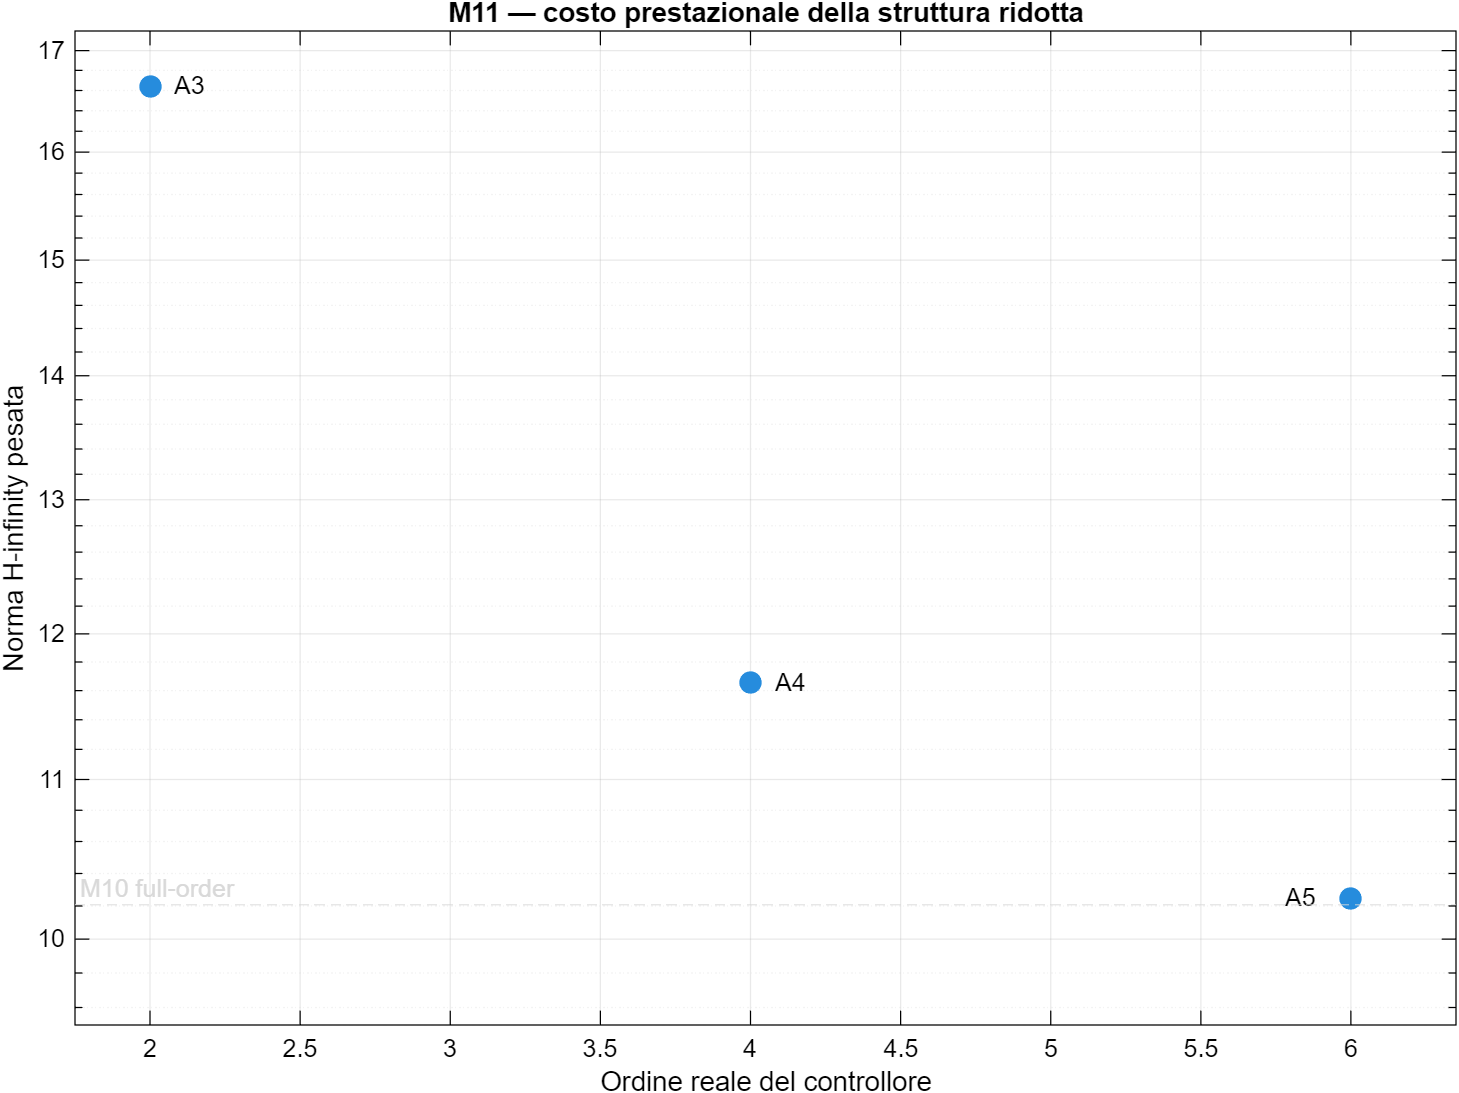
\includegraphics[width=0.80\textwidth]{figures/m11_gamma_vs_order.png}
\caption{Frontiera ordine--objective della baseline M11. Non sono risultati della nuova campagna a tre pesi.}
\label{fig:m11-order}
\end{figure}
La Figura~\ref{fig:m11-order} e la tabella seguente mantengono il confronto
storico. A5, ordine 6, è il candidato strutturato M12; non coincide
con $K_\infty$ M10, ordine 18.
% Tabella generata da build_m18_report_tables.m.
\begin{table}[H]
\centering
\begin{tabular}{lllll}
\toprule
Controllore & Ordine & $\gamma$/objective & NS & NP \\
\midrule
M9 mixsyn & 18 & 5.6772 & PASS & FAIL \\
M10 hinfsyn & 18 & 5.6772 & PASS & FAIL \\
M11 A3 & 2 & 8.1671 & PASS & FAIL \\
M11 A4 & 4 & 5.9672 & PASS & FAIL \\
M11 A5 & 6 & 5.7086 & PASS & FAIL \\
\bottomrule
\end{tabular}
\caption{Sintesi nominali H-infinity. Un valore $\gamma>1$ non costituisce PASS prestazionale.}
\label{tab:hinf}
\end{table}


La nuova campagna non modifica gli artifact o la pianta generalizzata
delle fasi M9--M16 originali. Poiché nessun nuovo candidato supera
l'insieme dei target e il comportamento incerto peggiora, non viene
adottato un nuovo peso nella catena di produzione. Non occorre
rieseguire M11, D--K, M14 o M16 per attribuire loro risultati nuovi
che non esistono. Se in futuro si promuovesse un nuovo controllore,
quelle verifiche dovrebbero essere ripetute sul problema corrispondente.
La sintesi nominale $H_\infty$ non sostituisce la successiva
$\mu$-analysis; neppure l'aggiunta di $W_3$ trasferisce automaticamente
al candidato il certificato di $K_\mu$.
